\KOMAoption{paper}{a4, portrait}
\areaset{267mm}{180mm}
\fancyheadoffset{0pt} % обновляем хедер и футер

\newgeometry{
  top=14mm,
  bottom=11mm,
  right=10mm,
  left=22mm,
}

\begin{landscape}

%\setlength{\headsep}{5.6mm} 
%\setlength{\topmargin}{-27mm}
\setlength{\footskip}{15.5pt}
%\setlength{\textwidth}{305mm}

\color{unimain}{\section[(справочное) Перечень сигналов ФСУ, предназначенных \newline для конфигурирования устройства <<ЮНИТ-М300-АРНТ>>]{(справочное)\\Перечень сигналов ФСУ, предназначенных для конфигурирования устройства <<ЮНИТ-М300-АРНТ>>}\label{app:signals}}
\color{black}

\begin{enumerate}[label=\ref{app:signals}.\arabic*] % Без глобального влияния
  \item Перечень сигналов самодиагностики, доступных для конфигурирования, приведен в документации ЮТКБ.656122.609 РЭ <<Устройство защиты и автоматики серии <<ЮНИТ-М300>>. Руководство по эксплуатации общее>>.
  \item Условные обозначения, применяемые в таблице перечня сигналов:
  \begin{itemize}
    \item[$\text{(--)}$] { - сигнал не имеет возможности конфигурации на данный параметр;}
    \item[$\text{(+)}$] { - сигнал имеет возможность конфигурации на данный параметр.}
  \end{itemize}
\end{enumerate}

\small % сделаем шрифт в таблице поменьше
% В таблице ниже убрал правую и левую горизонтальные линии чтобы не сливались и жирно видно - также в настройках geometry прищлось поле right =8mm а не 5 mm 
% так как строки ниже колонтитулов спускались
\begin{longtable}{
>{\centering\arraybackslash}m{6.0cm}
|>{\centering\arraybackslash}m{3.45cm}
|>{\centering\arraybackslash}m{2cm}
|>{\centering\arraybackslash}m{2cm}
|>{\centering\arraybackslash}m{2cm}
|>{\centering\arraybackslash}m{2cm}
|>{\centering\arraybackslash}m{2cm}
|>{\centering\arraybackslash}m{2cm}
|>{\centering\arraybackslash}m{2.107cm}
}

%\caption{Перечень сигналов ФСУ, предназначенных для конфигурирования устройств ЮНИТ-М300\vspace{-0.5\baselineskip}}\label{appA:tbl1}\\ % выравнивает надпись посередине таблицы
\caption{Перечень сигналов ФСУ, предназначенных для конфигурирования устройства\hfill\vspace{-0.5\baselineskip}}\label{appA:tbl1}\\ 

\hline
\rowcolor{unimain!40}
Полное наименование сигнала & Наименование сигнала на ФСУ & Дискретные входы & Выходные реле & Светодиоды & Функционал. клавиши & Регистратор событий & Аварийный осциллограф & Пуск авар. осциллографа \\ 
\hline
\endfirsthead
%\caption{\emph{Продолжение\vspace{-0.5\baselineskip}}} \\ % Отступ обозначения таблицы от таблицы и выравнивание надписи слева
\caption*{\hspace{3pt}\emph{Продолжение таблицы \ref{appA:tbl1}\hfill\vspace{-0.5\baselineskip}}} \\ % сделано по ГОСТ 2.105 п.6.8.7
\hline
\rowcolor{unimain!40}
Полное наименование сигнала & Наименование сигнала на ФСУ & Дискретные входы & Выходные реле & Светодиоды & Функционал. клавиши & Регистратор событий & Аварийный осциллограф & Пуск авар. осциллографа \\ 
%\hline
\endhead

%\hline
\endfoot

%\hline
\endlastfoot

%===t2
\rowcolor{gray!10}
\multicolumn{9}{c}{Общие сигналы ФС} \\
\hline
\raggedright Внешнее реле контроля тока РПН & \centering Внешн. РТ РПН & \centering + & \centering + & \centering + & \centering -- & \centering + & \centering + & \centering \arraybackslash + \\ \hline
\raggedright Отключенное положение автомата питания двигателя в приводе РПН & \centering бк автомата ПМ & \centering + & \centering + & \centering + & \centering -- & \centering + & \centering + & \centering \arraybackslash + \\ \hline
\raggedright Реле контроля низкой температуры масла РПН & \centering Реле низк. t РПН & \centering + & \centering + & \centering + & \centering -- & \centering + & \centering + & \centering \arraybackslash + \\ \hline
\raggedright Реле контроля низкого уровня масла РПН & \centering Реле низк .ур. масла & \centering + & \centering + & \centering + & \centering -- & \centering + & \centering + & \centering \arraybackslash + \\ \hline
\raggedright Ключ местное управление приводом РПН & \centering Ключ МУ РПН & \centering + & \centering + & \centering + & \centering -- & \centering + & \centering + & \centering \arraybackslash + \\ \hline
\raggedright Секция 1 включена & \centering Секция 1 включена & \centering + & \centering + & \centering + & \centering -- & \centering + & \centering + & \centering \arraybackslash + \\ \hline
\raggedright Секция 2 включена & \centering Секция 2 включена & \centering + & \centering + & \centering + & \centering -- & \centering + & \centering + & \centering \arraybackslash + \\ \hline
\raggedright Концевой выключатель сигнализации переключения привода РПН & \centering SQ переключение ПМ & \centering + & \centering + & \centering + & \centering -- & \centering + & \centering + & \centering \arraybackslash + \\ \hline
\raggedright Концевой выключатель верхнего положения РПН & \centering SQ верхн. полож. & \centering + & \centering + & \centering + & \centering -- & \centering + & \centering + & \centering \arraybackslash + \\ \hline
\raggedright Концевой выключатель нижнего положения РПН & \centering SQ нижн. полож. & \centering + & \centering + & \centering + & \centering -- & \centering + & \centering + & \centering \arraybackslash + \\ \hline
\raggedright АРНТ параллельного трансформатора в режиме авто & \centering Парал в режиме авто & \centering + & \centering + & \centering + & \centering -- & \centering + & \centering + & \centering \arraybackslash + \\ \hline
\raggedright АРНТ параллельного трансформатора принудительно ведущий & \centering Парал принуд ведущ & \centering + & \centering + & \centering + & \centering -- & \centering + & \centering + & \centering \arraybackslash + \\ \hline
\raggedright АРНТ параллельного трансформатора ведущий & \centering Парал. ведущий & \centering + & \centering + & \centering + & \centering -- & \centering + & \centering + & \centering \arraybackslash + \\ \hline
\raggedright Команда прибавить от АРНТ параллельного трансформатора & \centering Пар.рег.Прибав. & \centering + & \centering + & \centering + & \centering -- & \centering + & \centering + & \centering \arraybackslash + \\ \hline
\raggedright Команда убавить от АРНТ параллельного трансформатора & \centering Пар.рег.Убавить & \centering + & \centering + & \centering + & \centering -- & \centering + & \centering + & \centering \arraybackslash + \\ \hline
\raggedright Ненормальный режим на шинах параллельного трансформатора & \centering Парал ненорм режим & \centering + & \centering + & \centering + & \centering -- & \centering + & \centering + & \centering \arraybackslash + \\ \hline
\raggedright АРНТ параллельного трансформатора заблокирована & \centering Парал заблокирован & \centering + & \centering + & \centering + & \centering -- & \centering + & \centering + & \centering \arraybackslash + \\ \hline
\raggedright АРНТ параллельного трансформатора готов к режиму параллельного регулирования & \centering Парал. готовность & \centering + & \centering + & \centering + & \centering -- & \centering + & \centering + & \centering \arraybackslash + \\ \hline
\raggedright У параллельного трансформатора нет связи с регулируемыми шинами & \centering Парал. несоед. шины & \centering + & \centering + & \centering + & \centering -- & \centering + & \centering + & \centering \arraybackslash + \\ \hline
\raggedright Идет переключение привода РПН параллельного трансформатора & \centering Парал РПН переключ. & \centering + & \centering + & \centering + & \centering -- & \centering + & \centering + & \centering \arraybackslash + \\ \hline
\raggedright Внешний сигнал неисправности привода РПН & \centering Неисправность ПМ & \centering + & \centering + & \centering + & \centering -- & \centering + & \centering + & \centering \arraybackslash + \\ \hline
\raggedright Внешний сигнал рассогласования приводов РПН & \centering Внешн сигн рассогл & \centering + & \centering + & \centering + & \centering -- & \centering + & \centering + & \centering \arraybackslash + \\ \hline
\raggedright Положение блока испытательного №1 & \centering Вход SG1 & \centering + & \centering + & \centering + & \centering -- & \centering + & \centering + & \centering \arraybackslash + \\ \hline
\raggedright Положение блока испытательного №2 & \centering Вход SG2 & \centering + & \centering + & \centering + & \centering -- & \centering + & \centering + & \centering \arraybackslash + \\ \hline
\raggedright Положение блока испытательного №3 & \centering Вход SG3 & \centering + & \centering + & \centering + & \centering -- & \centering + & \centering + & \centering \arraybackslash + \\ \hline
\raggedright Положение блока испытательного №4 & \centering Вход SG4 & \centering + & \centering + & \centering + & \centering -- & \centering + & \centering + & \centering \arraybackslash + \\ \hline
\raggedright Положение блока испытательного №5 & \centering Вход SG5 & \centering + & \centering + & \centering + & \centering -- & \centering + & \centering + & \centering \arraybackslash + \\ \hline
\raggedright Положение блока испытательного №6 & \centering Вход SG6 & \centering + & \centering + & \centering + & \centering -- & \centering + & \centering + & \centering \arraybackslash + \\ \hline
\raggedright Положение блока испытательного №7 & \centering Вход SG7 & \centering + & \centering + & \centering + & \centering -- & \centering + & \centering + & \centering \arraybackslash + \\ \hline
\raggedright Концевой выключатель положения двери шкафа АРНТ & \centering SQ Дверь & \centering + & \centering + & \centering + & \centering -- & \centering + & \centering + & \centering \arraybackslash + \\ \hline
\raggedright Реле контроля оперативного тока технологической сигнализации РПН & \centering Опер. ток РПН & \centering + & \centering + & \centering + & \centering -- & \centering + & \centering + & \centering \arraybackslash + \\ \hline
\raggedright Сигнал BCD1 датчика положения РПН & \centering BCD1\_РПН & \centering + & \centering + & \centering + & \centering -- & \centering + & \centering + & \centering \arraybackslash + \\ \hline
\raggedright Сигнал BCD2 датчика положения РПН & \centering BCD2\_РПН & \centering + & \centering + & \centering + & \centering -- & \centering + & \centering + & \centering \arraybackslash + \\ \hline
\raggedright Сигнал BCD3 датчика положения РПН & \centering BCD3\_РПН & \centering + & \centering + & \centering + & \centering -- & \centering + & \centering + & \centering \arraybackslash + \\ \hline
\raggedright Сигнал BCD4 датчика положения РПН & \centering BCD4\_РПН & \centering + & \centering + & \centering + & \centering -- & \centering + & \centering + & \centering \arraybackslash + \\ \hline
\raggedright Сигнал BCD5 датчика положения РПН & \centering BCD5\_РПН & \centering + & \centering + & \centering + & \centering -- & \centering + & \centering + & \centering \arraybackslash + \\ \hline
\raggedright Сигнал BCD6 датчика положения РПН & \centering BCD6\_РПН & \centering + & \centering + & \centering + & \centering -- & \centering + & \centering + & \centering \arraybackslash + \\ \hline
\raggedright Сигнал BCD1 датчика положения РПН параллельного трансформатора & \centering BCD1\_парал\_РПН & \centering + & \centering + & \centering + & \centering -- & \centering + & \centering + & \centering \arraybackslash + \\ \hline
\raggedright Сигнал BCD2 датчика положения РПН параллельного трансформатора & \centering BCD2\_парал\_РПН & \centering + & \centering + & \centering + & \centering -- & \centering + & \centering + & \centering \arraybackslash + \\ \hline
\raggedright Сигнал BCD3 датчика положения РПН параллельного трансформатора & \centering BCD3\_парал\_РПН & \centering + & \centering + & \centering + & \centering -- & \centering + & \centering + & \centering \arraybackslash + \\ \hline
\raggedright Сигнал BCD4 датчика положения РПН параллельного трансформатора & \centering BCD4\_парал\_РПН & \centering + & \centering + & \centering + & \centering -- & \centering + & \centering + & \centering \arraybackslash + \\ \hline
\raggedright Сигнал BCD5 датчика положения РПН параллельного трансформатора & \centering BCD5\_парал\_РПН & \centering + & \centering + & \centering + & \centering -- & \centering + & \centering + & \centering \arraybackslash + \\ \hline
\raggedright Сигнал BCD6 датчика положения РПН параллельного трансформатора & \centering BCD6\_парал\_РПН & \centering + & \centering + & \centering + & \centering -- & \centering + & \centering + & \centering \arraybackslash + \\ \hline
\raggedright Внутренняя неисправность & \centering IRF & \centering + & \centering + & \centering + & \centering -- & \centering + & \centering + & \centering \arraybackslash + \\ \hline
\raggedright Test/blocked & \centering Test/blocked & \centering + & \centering + & \centering + & \centering -- & \centering + & \centering + & \centering \arraybackslash + \\ \hline
\raggedright Поведение местного управления & \centering Повед. местн. упр. & \centering + & \centering + & \centering + & \centering -- & \centering + & \centering + & \centering \arraybackslash + \\ \hline
\raggedright Положение ключа режима управления & \centering Ключ упр. & \centering + & \centering + & \centering + & \centering -- & \centering + & \centering + & \centering \arraybackslash + \\ \hline
\raggedright Право на переключение на уровне станции & \centering Перекл. ур. станц. & \centering + & \centering + & \centering + & \centering -- & \centering + & \centering + & \centering \arraybackslash + \\ \hline
\raggedright Критическая неисправность & \centering Неисправность & \centering + & \centering -- & \centering + & \centering -- & \centering + & \centering + & \centering \arraybackslash + \\ \hline
\raggedright Некритическая ошибка & \centering Ошибка & \centering + & \centering -- & \centering + & \centering -- & \centering + & \centering + & \centering \arraybackslash + \\ \hline
\raggedright Вывод терминала от ФК & \centering ФК: Вывод терминала & \centering -- & \centering -- & \centering + & \centering + & \centering + & \centering + & \centering \arraybackslash + \\ \hline
\raggedright Вывод терминала от ДВ & \centering ДВ: Вывод терминала & \centering + & \centering -- & \centering -- & \centering -- & \centering + & \centering + & \centering \arraybackslash + \\ \hline
\raggedright Ввод режима автоматического регулирования от ФК & \centering ФК: Ввод режима авто & \centering -- & \centering -- & \centering + & \centering + & \centering + & \centering + & \centering \arraybackslash + \\ \hline
\raggedright Ввод режима автоматического регулирования от ДВ & \centering ДВ: Ввод режима авто & \centering + & \centering -- & \centering -- & \centering -- & \centering + & \centering + & \centering \arraybackslash + \\ \hline
\raggedright Ввод режима автоматического выбора регулируемой секции от ФК & \centering ФК: Ввод авт.выбор секц & \centering -- & \centering -- & \centering + & \centering + & \centering + & \centering + & \centering \arraybackslash + \\ \hline
\raggedright Ввод режима автоматического выбора регулируемой секции от ДВ & \centering ДВ: Ввод авт.выбор секц & \centering + & \centering -- & \centering -- & \centering -- & \centering + & \centering + & \centering \arraybackslash + \\ \hline
\raggedright Ввод режима приоритета регулирования по 2 секции от ФК & \centering ФК: Ввод рег. по 2 секц & \centering -- & \centering -- & \centering + & \centering + & \centering + & \centering + & \centering \arraybackslash + \\ \hline
\raggedright Ввод режима приоритета регулирования по 2 секции от ДВ & \centering ДВ: Ввод рег. по 2 секц & \centering + & \centering -- & \centering -- & \centering -- & \centering + & \centering + & \centering \arraybackslash + \\ \hline
\raggedright Ввод режима параллельного регулирования трансформаторов от ФК & \centering ФК: Ввод парал. рег. & \centering -- & \centering -- & \centering + & \centering + & \centering + & \centering + & \centering \arraybackslash + \\ \hline
\raggedright Ввод режима параллельного регулирования трансформаторов от ДВ & \centering ДВ: Ввод парал. рег. & \centering + & \centering -- & \centering -- & \centering -- & \centering + & \centering + & \centering \arraybackslash + \\ \hline
\raggedright Команда сброс от ФК & \centering ФК: Сброс & \centering -- & \centering -- & \centering + & \centering + & \centering + & \centering + & \centering \arraybackslash + \\ \hline
\raggedright Команда сброс от ДВ & \centering ДВ: Сброс & \centering + & \centering -- & \centering -- & \centering -- & \centering + & \centering + & \centering \arraybackslash + \\ \hline
\raggedright Ручная команда прибавить от ФК & \centering ФК: КУ Прибавить & \centering -- & \centering -- & \centering + & \centering + & \centering + & \centering + & \centering \arraybackslash + \\ \hline
\raggedright Ручная команда прибавить от ДВ & \centering ДВ: КУ Прибавить & \centering + & \centering -- & \centering -- & \centering -- & \centering + & \centering + & \centering \arraybackslash + \\ \hline
\raggedright Ручная команда убавить от ФК & \centering ФК: КУ Убавить & \centering -- & \centering -- & \centering + & \centering + & \centering + & \centering + & \centering \arraybackslash + \\ \hline
\raggedright Ручная команда убавить от ДВ & \centering ДВ: КУ Убавить & \centering + & \centering -- & \centering -- & \centering -- & \centering + & \centering + & \centering \arraybackslash + \\ \hline
\raggedright Команда сброс счетчика на начальное значение от ФК & \centering ФК: Сброс счет. перекл. & \centering -- & \centering -- & \centering + & \centering + & \centering + & \centering + & \centering \arraybackslash + \\ \hline
\raggedright Команда сброс счетчика на начальное значение от ДВ & \centering ДВ: Сброс счет. перекл. & \centering + & \centering -- & \centering -- & \centering -- & \centering + & \centering + & \centering \arraybackslash + \\ \hline
\raggedright Команда сброс счетчика положений РПН на значение по умолчанию от ФК & \centering ФК: Сброс Сч.Полож. & \centering -- & \centering -- & \centering + & \centering + & \centering + & \centering + & \centering \arraybackslash + \\ \hline
\raggedright Команда сброс счетчика положений РПН на значение по умолчанию от ДВ & \centering ДВ: Сброс Сч.Полож. & \centering + & \centering -- & \centering -- & \centering -- & \centering + & \centering + & \centering \arraybackslash + \\ \hline
\rowcolor{gray!10}
\multicolumn{9}{c}{Автоматическое регулирования напряжения трансформатора (АРНТ)} \\
\hline
\raggedright Автоматический выбор регулируемой секции & \centering АРНТ\_Авто выбор секц & \centering -- & \centering + & \centering + & \centering -- & \centering + & \centering + & \centering \arraybackslash + \\ \hline
\raggedright Приоритет регулирования по 2 секции & \centering АРНТ\_Приоритет 2 секц & \centering -- & \centering + & \centering + & \centering -- & \centering + & \centering + & \centering \arraybackslash + \\ \hline
\raggedright Нет связи с регулируемыми шинами & \centering АРНТ\_Нет связи с шинами & \centering -- & \centering + & \centering + & \centering -- & \centering + & \centering + & \centering \arraybackslash + \\ \hline
\raggedright Запрет автоматического повышения при перегрузке & \centering АРНТ\_Перегрузка & \centering -- & \centering + & \centering + & \centering -- & \centering + & \centering + & \centering \arraybackslash + \\ \hline
\raggedright Запрет автоматического повышения при перенапряжении & \centering АРНТ\_Высокое U секц & \centering -- & \centering + & \centering + & \centering -- & \centering + & \centering + & \centering \arraybackslash + \\ \hline
\raggedright Запрет авторегулирования при низком напряжении & \centering АРНТ\_Низкое U секц & \centering -- & \centering + & \centering + & \centering -- & \centering + & \centering + & \centering \arraybackslash + \\ \hline
\raggedright Запрет автоматического повышения при высоком напряжении НП & \centering АРНТ\_Высокое 3U0 & \centering -- & \centering + & \centering + & \centering -- & \centering + & \centering + & \centering \arraybackslash + \\ \hline
\raggedright Запрет авторегулирования при высоком напряжении ОП & \centering АРНТ\_Высокое U2 & \centering -- & \centering + & \centering + & \centering -- & \centering + & \centering + & \centering \arraybackslash + \\ \hline
\raggedright Ненормальный режим на секции & \centering АРНТ\_Ненормальный режим & \centering -- & \centering + & \centering + & \centering -- & \centering + & \centering + & \centering \arraybackslash + \\ \hline
\raggedright Блокировка РПН по току & \centering АРНТ\_Блокир. по току РПН & \centering -- & \centering + & \centering + & \centering -- & \centering + & \centering + & \centering \arraybackslash + \\ \hline
\raggedright Отключено питание привода РПН & \centering АРНТ\_Отключен автомат ПМ & \centering -- & \centering + & \centering + & \centering -- & \centering + & \centering + & \centering \arraybackslash + \\ \hline
\raggedright Блокировка РПН по низкой температуре & \centering АРНТ\_Блок.по температуре & \centering -- & \centering + & \centering + & \centering -- & \centering + & \centering + & \centering \arraybackslash + \\ \hline
\raggedright Блокировка РПН по низкому уровню масла & \centering АРНТ\_Блок.по уров. масла & \centering -- & \centering + & \centering + & \centering -- & \centering + & \centering + & \centering \arraybackslash + \\ \hline
\raggedright Привод РПН в местном управлении & \centering АРНТ\_ПМ в местном упр & \centering -- & \centering + & \centering + & \centering -- & \centering + & \centering + & \centering \arraybackslash + \\ \hline
\raggedright Привод РПН заблокирован & \centering АРНТ\_ПМ заблокирован & \centering -- & \centering + & \centering + & \centering -- & \centering + & \centering + & \centering \arraybackslash + \\ \hline
\raggedright Напряжение ниже границы зоны нечувствительности & \centering АРНТ\_Напряжение ниже & \centering -- & \centering + & \centering + & \centering -- & \centering + & \centering + & \centering \arraybackslash + \\ \hline
\raggedright Напряжение выше границы зоны нечувствительности & \centering АРНТ\_Напряжение выше & \centering -- & \centering + & \centering + & \centering -- & \centering + & \centering + & \centering \arraybackslash + \\ \hline
\raggedright Напряжение значительно выше границы зоны нечувствительности & \centering АРНТ\_Знач.повыш.напряж. & \centering -- & \centering + & \centering + & \centering -- & \centering + & \centering + & \centering \arraybackslash + \\ \hline
\raggedright Ошибка определения положения РПН & \centering АРНТ\_Ошибка полож. РПН & \centering -- & \centering + & \centering + & \centering -- & \centering + & \centering + & \centering \arraybackslash + \\ \hline
\raggedright Привод РПН в крайнем верхнем положении & \centering АРНТ\_Крайн.верх.полож. & \centering -- & \centering + & \centering + & \centering -- & \centering + & \centering + & \centering \arraybackslash + \\ \hline
\raggedright Привод РПН в крайнем нижнем положении & \centering АРНТ\_Крайн.нижн.полож. & \centering -- & \centering + & \centering + & \centering -- & \centering + & \centering + & \centering \arraybackslash + \\ \hline
\raggedright Промежуточное положение привода РПН & \centering АРНТ\_Промежут полож & \centering -- & \centering + & \centering + & \centering -- & \centering + & \centering + & \centering \arraybackslash + \\ \hline
\raggedright Блокировка автоматической команды прибавить по верхнему допустимому положению & \centering АРНТ\_Блок.Верх.Полож. & \centering -- & \centering + & \centering + & \centering -- & \centering + & \centering + & \centering \arraybackslash + \\ \hline
\raggedright Блокировка автоматической команды убавить по нижнему допустимому положению & \centering АРНТ\_Блок.Нижн.Полож. & \centering -- & \centering + & \centering + & \centering -- & \centering + & \centering + & \centering \arraybackslash + \\ \hline
\raggedright Неисправность РПН & \centering АРНТ\_Неисправность РПН & \centering -- & \centering + & \centering + & \centering -- & \centering + & \centering + & \centering \arraybackslash + \\ \hline
\raggedright Привод РПН не начал переключение & \centering АРНТ\_ПМ не пошел & \centering -- & \centering + & \centering + & \centering -- & \centering + & \centering + & \centering \arraybackslash + \\ \hline
\raggedright Привод РПН не завершил переключение & \centering АРНТ\_ПМ застрял & \centering -- & \centering + & \centering + & \centering -- & \centering + & \centering + & \centering \arraybackslash + \\ \hline
\raggedright Привод РПН самопроизвольно переключился & \centering АРНТ\_ПМ побежал & \centering -- & \centering + & \centering + & \centering -- & \centering + & \centering + & \centering \arraybackslash + \\ \hline
\raggedright Привод РПН в процессе переключения & \centering АРНТ\_Переключение & \centering -- & \centering + & \centering + & \centering -- & \centering + & \centering + & \centering \arraybackslash + \\ \hline
\raggedright Сигнализация максимального количества переключений РПН & \centering АРНТ\_Ресурс исчерпан & \centering -- & \centering + & \centering + & \centering -- & \centering + & \centering + & \centering \arraybackslash + \\ \hline
\raggedright Команда на отключение питания привода РПН & \centering АРНТ\_Отключение ПМ & \centering -- & \centering + & \centering + & \centering -- & \centering + & \centering + & \centering \arraybackslash + \\ \hline
\raggedright Режим автоматического регулирования & \centering АРНТ\_Режим авто. регул. & \centering -- & \centering + & \centering + & \centering -- & \centering + & \centering + & \centering \arraybackslash + \\ \hline
\raggedright Управление заблокировано & \centering АРНТ\_Управл. блок. & \centering -- & \centering + & \centering + & \centering -- & \centering + & \centering + & \centering \arraybackslash + \\ \hline
\raggedright Команда прибавить в привод РПН & \centering АРНТ\_Прибавить & \centering -- & \centering + & \centering + & \centering -- & \centering + & \centering + & \centering \arraybackslash + \\ \hline
\raggedright Команда убавить в привод РПН & \centering АРНТ\_Убавить & \centering -- & \centering + & \centering + & \centering -- & \centering + & \centering + & \centering \arraybackslash + \\ \hline
\raggedright Режим параллельного регулирования & \centering АРНТ\_Режим парал. регул & \centering -- & \centering + & \centering + & \centering -- & \centering + & \centering + & \centering \arraybackslash + \\ \hline
\raggedright Готовность к режиму параллельного регулирования трансформаторов & \centering АРНТ\_Готов к парал. рег. & \centering -- & \centering + & \centering + & \centering -- & \centering + & \centering + & \centering \arraybackslash + \\ \hline
\raggedright Ведущий в режиме параллельного регулирования трансформаторов & \centering АРНТ\_Ведущий & \centering -- & \centering + & \centering + & \centering -- & \centering + & \centering + & \centering \arraybackslash + \\ \hline
\raggedright Принудительно ведущий в режиме параллельного регулирования трансформаторов & \centering АРНТ\_Принудит. ведущий & \centering -- & \centering + & \centering + & \centering -- & \centering + & \centering + & \centering \arraybackslash + \\ \hline
\raggedright Ведомый в режиме параллельного регулирования трансформаторов & \centering АРНТ\_Ведомый & \centering -- & \centering + & \centering + & \centering -- & \centering + & \centering + & \centering \arraybackslash + \\ \hline
\raggedright Параллельное регулирование заблокировано & \centering АРНТ\_Парал. рег. заблок & \centering -- & \centering + & \centering + & \centering -- & \centering + & \centering + & \centering \arraybackslash + \\ \hline
\raggedright Ошибка параллельного регулирования трансформаторов & \centering АРНТ\_Ошибка парал. рег. & \centering -- & \centering + & \centering + & \centering -- & \centering + & \centering + & \centering \arraybackslash + \\ \hline
\raggedright Прибавить в АРНТ параллельного трансформатора & \centering АРНТ\_Прибавить в парал. & \centering -- & \centering + & \centering + & \centering -- & \centering + & \centering + & \centering \arraybackslash + \\ \hline
\raggedright Убавить в АРНТ параллельного трансформатора & \centering АРНТ\_Убавить в парал. & \centering -- & \centering + & \centering + & \centering -- & \centering + & \centering + & \centering \arraybackslash + \\ \hline
\raggedright Рассогласование приводов РПН параллельных трансформаторов & \centering АРНТ\_Рассогласование РПН & \centering -- & \centering + & \centering + & \centering -- & \centering + & \centering + & \centering \arraybackslash + \\ \hline
\raggedright Блок испытательный №1 в рабочем положении & \centering АРНТ\_БИ 1 в работе & \centering -- & \centering + & \centering + & \centering -- & \centering + & \centering + & \centering \arraybackslash + \\ \hline
\raggedright Блок испытательный №2 в рабочем положении & \centering АРНТ\_БИ 2 в работе & \centering -- & \centering + & \centering + & \centering -- & \centering + & \centering + & \centering \arraybackslash + \\ \hline
\raggedright Блок испытательный №3 в рабочем положении & \centering АРНТ\_БИ 3 в работе & \centering -- & \centering + & \centering + & \centering -- & \centering + & \centering + & \centering \arraybackslash + \\ \hline
\raggedright Блок испытательный №4 в рабочем положении & \centering АРНТ\_БИ 4 в работе & \centering -- & \centering + & \centering + & \centering -- & \centering + & \centering + & \centering \arraybackslash + \\ \hline
\raggedright Блок испытательный №5 в рабочем положении & \centering АРНТ\_БИ 5 в работе & \centering -- & \centering + & \centering + & \centering -- & \centering + & \centering + & \centering \arraybackslash + \\ \hline
\raggedright Блок испытательный №6 в рабочем положении & \centering АРНТ\_БИ 6 в работе & \centering -- & \centering + & \centering + & \centering -- & \centering + & \centering + & \centering \arraybackslash + \\ \hline
\raggedright Блок испытательный №7 в рабочем положении & \centering АРНТ\_БИ 7 в работе & \centering -- & \centering + & \centering + & \centering -- & \centering + & \centering + & \centering \arraybackslash + \\ \hline
\raggedright Блок испытательный не в рабочем положении & \centering АРНТ\_БИ выведены & \centering -- & \centering + & \centering + & \centering -- & \centering + & \centering + & \centering \arraybackslash + \\ \hline
\raggedright Дверь шкафа АРНТ закрыта & \centering АРНТ\_Дверь закрыта & \centering -- & \centering + & \centering + & \centering -- & \centering + & \centering + & \centering \arraybackslash + \\ \hline
\raggedright Дверь шкафа АРНТ открыта & \centering АРНТ\_Дверь открыта & \centering -- & \centering + & \centering + & \centering -- & \centering + & \centering + & \centering \arraybackslash + \\ \hline
\raggedright Неисправность оперативного тока цепей технологической сигнализации & \centering АРНТ\_Неиспр. опер. тока & \centering -- & \centering + & \centering + & \centering -- & \centering + & \centering + & \centering \arraybackslash + \\ \hline
\raggedright Предупредительная сигнализация & \centering АРНТ\_Предупр. сигнал. & \centering -- & \centering + & \centering + & \centering -- & \centering + & \centering + & \centering \arraybackslash + \\ \hline
\raggedright Функция АРНТ в работе & \centering АРНТ\_АРНТ в работе & \centering -- & \centering + & \centering + & \centering -- & \centering + & \centering + & \centering \arraybackslash + \\ \hline
\rowcolor{gray!10}
\multicolumn{9}{c}{ВКл: Вывод терминала} \\
\hline
\raggedright Оперативный вывод функции & \centering Виртуальный ключ-1\_Опер. вывод & \centering -- & \centering + & \centering + & \centering -- & \centering + & \centering + & \centering \arraybackslash + \\ \hline
\rowcolor{gray!10}
\multicolumn{9}{c}{ВКл: Ввод режима авто} \\
\hline
\raggedright Оперативный вывод функции & \centering Виртуальный ключ-2\_Опер. вывод & \centering -- & \centering + & \centering + & \centering -- & \centering + & \centering + & \centering \arraybackslash + \\ \hline
\rowcolor{gray!10}
\multicolumn{9}{c}{ВКл: Ввод авт.выбор секц} \\
\hline
\raggedright Оперативный вывод функции & \centering Виртуальный ключ-3\_Опер. вывод & \centering -- & \centering + & \centering + & \centering -- & \centering + & \centering + & \centering \arraybackslash + \\ \hline
\rowcolor{gray!10}
\multicolumn{9}{c}{ВКл: Ввод рег. по 2 секц} \\
\hline
\raggedright Оперативный вывод функции & \centering Виртуальный ключ-4\_Опер. вывод & \centering -- & \centering + & \centering + & \centering -- & \centering + & \centering + & \centering \arraybackslash + \\ \hline
\rowcolor{gray!10}
\multicolumn{9}{c}{ВКл: Ввод парал. рег.} \\
\hline
\raggedright Оперативный вывод функции & \centering Виртуальный ключ-5\_Опер. вывод & \centering -- & \centering + & \centering + & \centering -- & \centering + & \centering + & \centering \arraybackslash + \\ \hline
\rowcolor{gray!10}
\multicolumn{9}{c}{ВКн: Сброс} \\
\hline
\raggedright Оперативный сброс функции & \centering Виртуальная кнопка-1\_Опер. сброс & \centering -- & \centering + & \centering + & \centering -- & \centering + & \centering + & \centering \arraybackslash + \\ \hline
\rowcolor{gray!10}
\multicolumn{9}{c}{ВКн: КУ Прибавить} \\
\hline
\raggedright Оперативный сброс функции & \centering Виртуальная кнопка-2\_Опер. сброс & \centering -- & \centering + & \centering + & \centering -- & \centering + & \centering + & \centering \arraybackslash + \\ \hline
\rowcolor{gray!10}
\multicolumn{9}{c}{ВКн: КУ Убавить} \\
\hline
\raggedright Оперативный сброс функции & \centering Виртуальная кнопка-3\_Опер. сброс & \centering -- & \centering + & \centering + & \centering -- & \centering + & \centering + & \centering \arraybackslash + \\ \hline
\rowcolor{gray!10}
\multicolumn{9}{c}{ВКн: Сброс счет. перекл.} \\
\hline
\raggedright Оперативный сброс функции & \centering Виртуальная кнопка-4\_Опер. сброс & \centering -- & \centering + & \centering + & \centering -- & \centering + & \centering + & \centering \arraybackslash + \\ \hline
\rowcolor{gray!10}
\multicolumn{9}{c}{ВКн: Сброс Сч.Полож.} \\
\hline
\raggedright Оперативный сброс функции & \centering Виртуальная кнопка-5\_Опер. сброс & \centering -- & \centering + & \centering + & \centering -- & \centering + & \centering + & \centering \arraybackslash + \\ \hline
%===t2
\end{longtable} 

\clearpage
\normalsize
%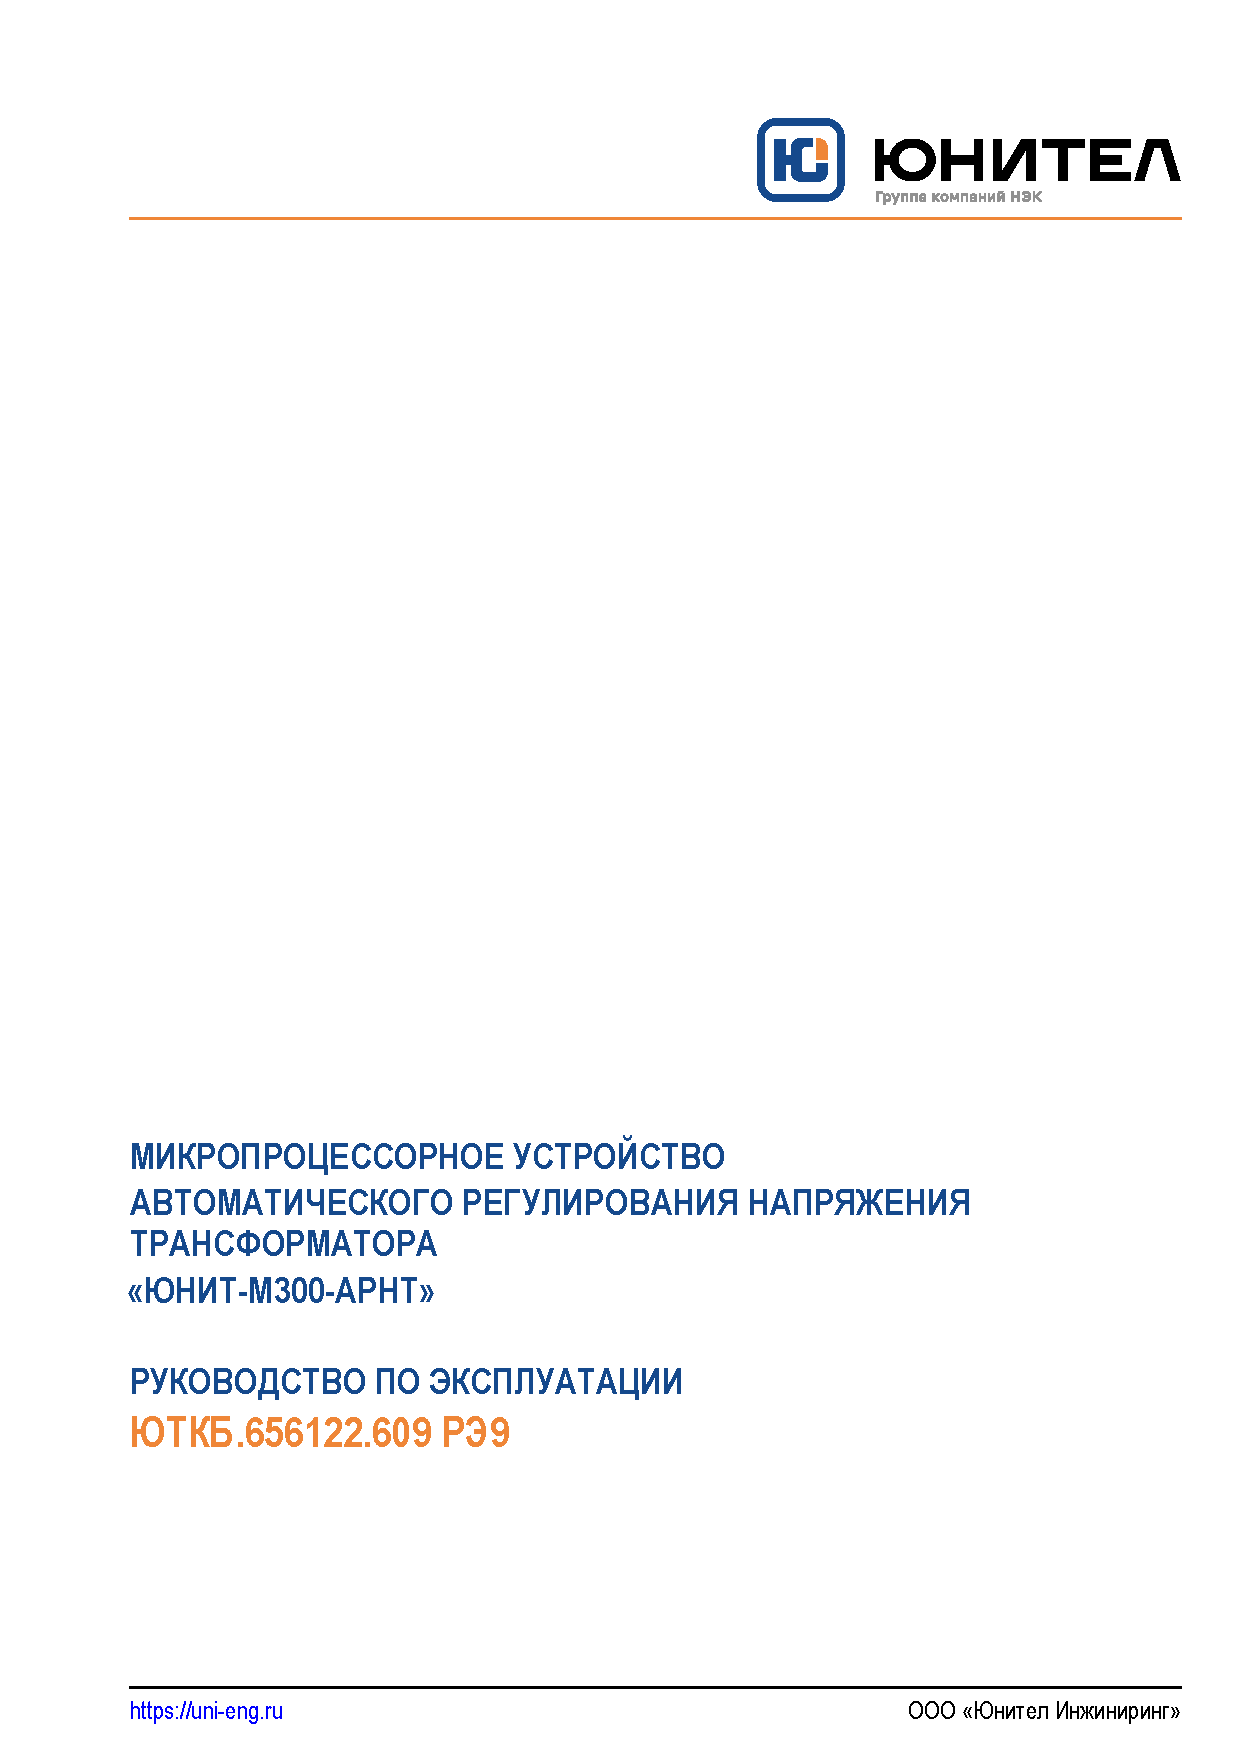
\includepdf[pages={1},width=0.5\textwidth, angle=90]{1.pdf} вставляем и поворачиваем pdf
%\begin{center}
%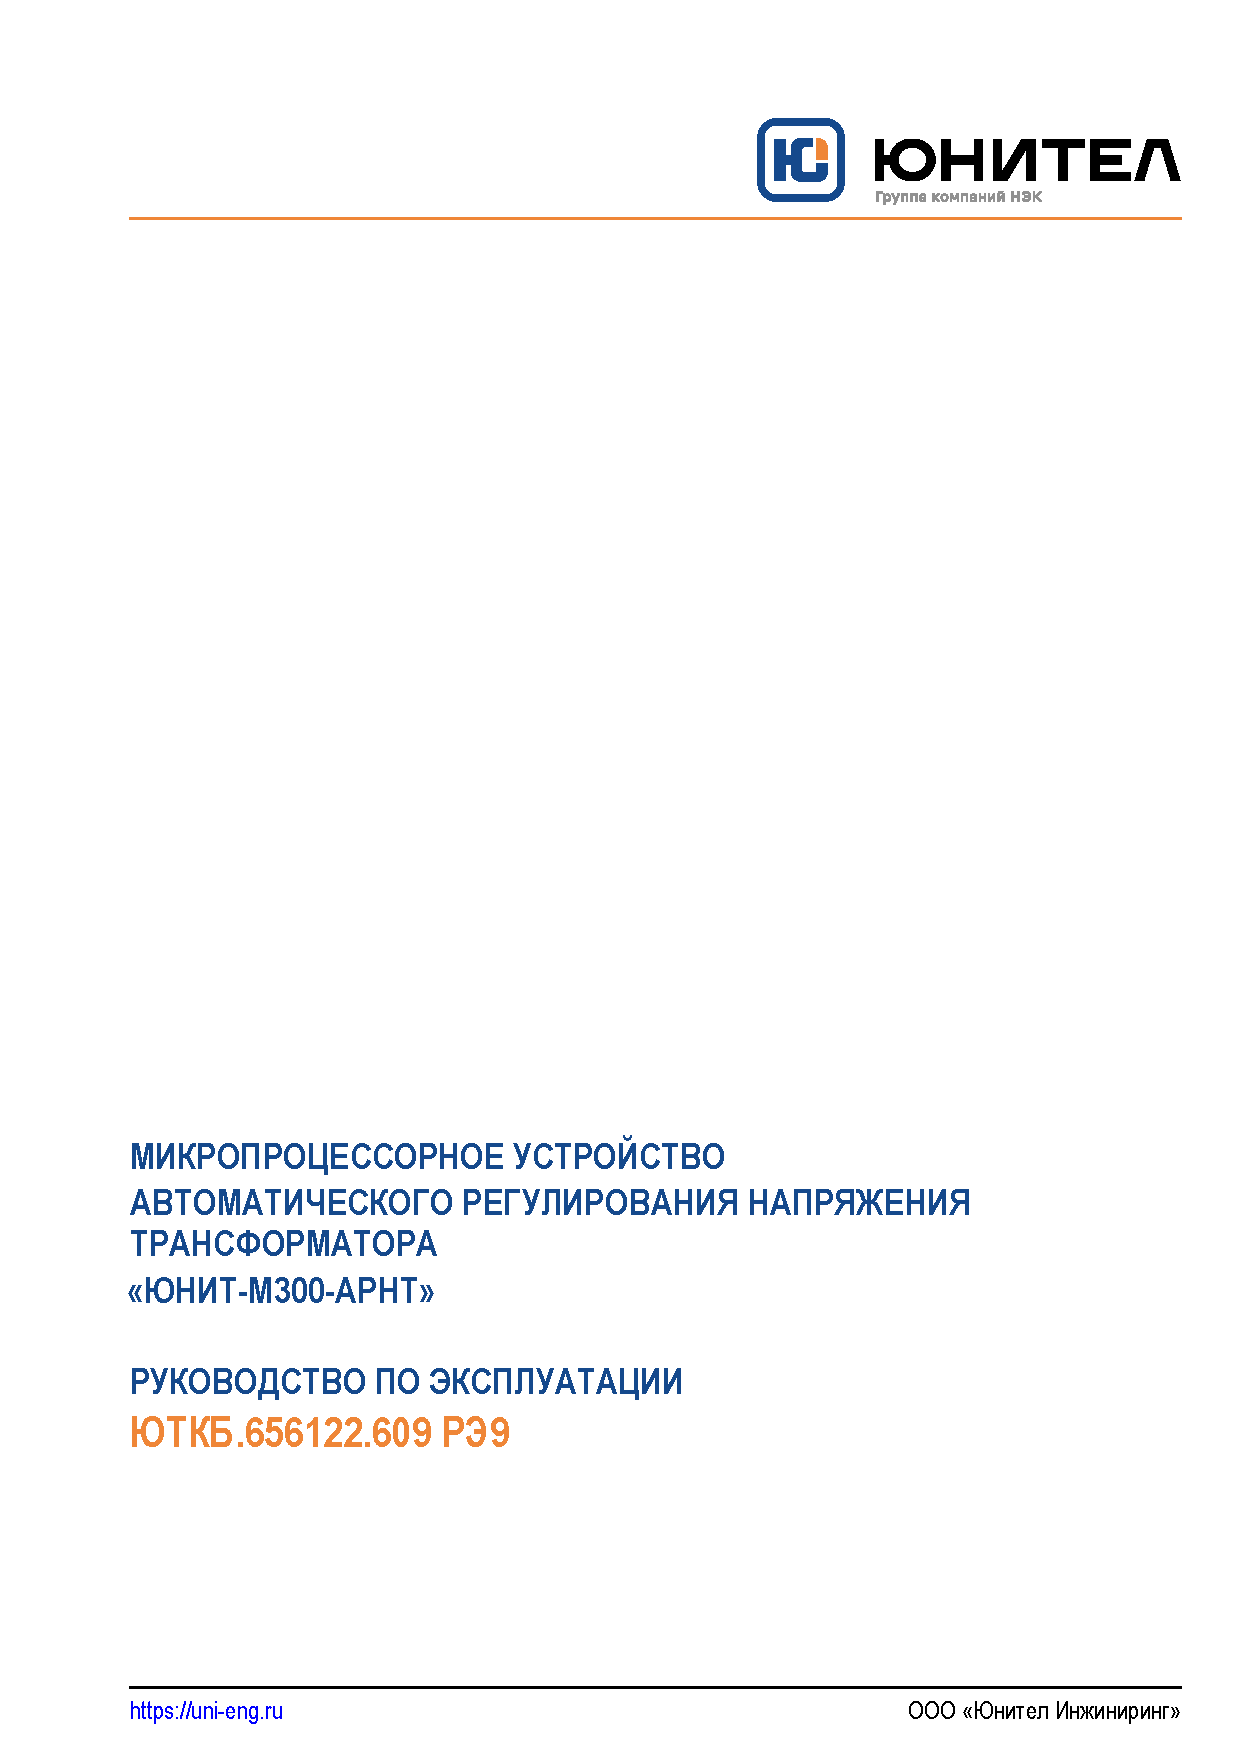
\includegraphics[width=1.4\textwidth]{1.pdf}
%\end{center}

\end{landscape}
\restoregeometry
